\documentclass{beamer}
\usepackage{xcolor}
\usepackage{natbib} % package to organize literature
\usepackage{multicol}
\usepackage{booktabs}
\usepackage{wasysym} % additional symbols
\usepackage{graphicx} % to include graphics, gifs
\usepackage{color} % add colored text
\usepackage{lmodern} % to fix font size error, might be problematic with math symbols
\usepackage{array}
\usepackage{tikz}
\usepackage{enumerate}
\usepackage{arydshln} % dashed lines

% Custom beamer settings
\definecolor{beamer@sbred}{rgb}{0.65,0.15,0.18}
%\definecolor{beamer@sbred}{rgb}{0.22,0.22,0.66}
%\setbeamercolor{title}{fg=beamer@sbred,bg=black!5}
\setbeamercolor{structure}{fg=beamer@sbred}
\setbeamercolor{frametitle}{fg=beamer@sbred}
\setbeamercolor{palette primary}{fg=beamer@sbred,bg=black!10}
\setbeamercolor{palette secondary}{fg=beamer@sbred}
\setbeamercolor{palette tertiary}{bg=beamer@sbred}
\setbeamercolor{palette quaternary}{fg=white,bg=beamer@sbred}
\setbeamertemplate{itemize items}[default]
\setbeamertemplate{enumerate items}[default]
\setbeamersize{text margin left=1em,text margin right=1em}
\DeclareTextFontCommand{\emph}{\color{beamer@sbred}}
\setbeamercolor*{block title example}{fg= white, bg= beamer@sbred!90}
\setbeamercolor*{block body example}{fg= black, bg= beamer@sbred!10}


\author{Patrick W. Kraft}
\institute{113\textsuperscript{th} APSA Annual Meeting}
\title{Looking for Answers\\{\large A Naive Approach for Measuring Political Sophistication}}
\date{San Francisco, 1 September 2017}
\titlegraphic{\includegraphics[height=.7cm]{/data/Dropbox/Uni/Misc/Logos/logo.pdf}}

\begin{document}
\frame{\titlepage}
%\footnotesize
% Thank you very much, my name is Patrick Kraft and I am a PhD Candidate at the Department for Political Science at Stony Brook University. The paper I am presenting today proposes a new measure of political sophistication based on verbatim attitude expression in open-ended survey items. Most studies that are interested in political sophistication focus on conventional factual knowledge scores as proxies. However, these measures have been criticized from theoretical and measurement perspectives. Lupia, for example, argues that the factual information asked for often has now apparent relevance to perform political tasks. The approach that I propose is naive in that it does not presuppose a set of information that is deemed necessary. Rather, it tries to quantify the complexity of individual attitude expressions related to a political task.


\section{Introduction}

\begin{frame}%[allowframebreaks]
\frametitle{Who scores higher on political knowledge?}
\begin{table}[ht]\footnotesize\centering
\begin{tabular}{l|p{4.5cm}|p{4.5cm}}
   \toprule
%  & Low Sophistication Response & High Sophistication Response \\ 
    & \textbf{Respondent A} & \textbf{Respondent B} \\ 
    \midrule
  Obama (+) & \textcolor{white}{I think he is honest, has good intentions.} & \textcolor{white}{He's got a hot wife. Sound mind. Bill Clinton, the best president we ever had, is voting for him. He's not in any type of scandal and is the perfect president for us now.} \\ \hdashline
  Obama (-) & \textcolor{white}{I don't feel he is up for the job, he doesn't really know how to get things accomplished from idea to actual reality.} &  \\ \hdashline
  Romney (+) & \textcolor{white}{He comes across as an honest person and I feel that financially he would be better for the country.} &  \\ \hdashline
  Romney (-) & \textcolor{white}{I am a moderate conservative and there are some things about anti-gay rights that I don't support.} & \textcolor{white}{Everything.} \\
    \bottomrule
 \end{tabular}
\end{table}
\end{frame}
% OLD: I am interested in how individuals describe and justify their political attitudes, which can have important effects, especially in a social context. In my dissertation, I work a lot with open-ended responses.
% OLD: mention data source: ANES 2012, around 5000 respondents, online + f2f study
% I want to start with a little example. I am going to show you two sample responses to open-ended likes/dislikes items in the 2012 American National Election Study. Respondent A and B both described what they liked and disliked about the two major presidential candidates, Barack Obama and Mitt Romney. You know, back in the good old days when Presidential candidates were not considered completely crazy. Respondent A said the following:

\begin{frame}%[allowframebreaks]
\frametitle{Who scores higher on political knowledge?}
\begin{table}[ht]\footnotesize\centering
\begin{tabular}{l|p{4.5cm}|p{4.5cm}}
   \toprule
%  & Low Sophistication Response & High Sophistication Response \\ 
    & \textbf{Respondent A} & \textbf{Respondent B} \\ 
    \midrule
  Obama (+) & I think he is honest, has good intentions. & \textcolor{white}{He's got a hot wife. Sound mind. Bill Clinton, the best president we ever had, is voting for him. He's not in any type of scandal and is the perfect president for us now.} \\ \hdashline
  Obama (-) & I don't feel he is up for the job, he doesn't really know how to get things accomplished from idea to actual reality. &  \\ \hdashline
  Romney (+) & He comes across as an honest person and I feel that financially he would be better for the country. &  \\ \hdashline
  Romney (-) & I am a moderate conservative and there are some things about anti-gay rights that I don't support. & \textcolor{white}{Everything.} \\
    \bottomrule
 \end{tabular}
\end{table}
\end{frame}
% ... Respondent B, on the other hand, said...

\begin{frame}%[allowframebreaks]
\frametitle{Who scores higher on political knowledge?}
\begin{table}[ht]\footnotesize\centering
\begin{tabular}{l|p{4.5cm}|p{4.5cm}}
   \toprule
%  & Low Sophistication Response & High Sophistication Response \\ 
    & \textbf{Respondent A} & \textbf{Respondent B} \\ 
    \midrule
  Obama (+) & I think he is honest, has good intentions. & He's got a hot wife. Sound mind. Bill Clinton, the best president we ever had, is voting for him. He's not in any type of scandal and is the perfect president for us now. \\ \hdashline
  Obama (-) & I don't feel he is up for the job, he doesn't really know how to get things accomplished from idea to actual reality. &  \\ \hdashline
  Romney (+) & He comes across as an honest person and I feel that financially he would be better for the country. &  \\ \hdashline
  Romney (-) & I am a moderate conservative and there are some things about anti-gay rights that I don't support. & Everything. \\
    \bottomrule
 \end{tabular}
\end{table}
\end{frame}
% Now, who would you guess scored higher in factual political knowledge? Clearly, our intuition tells us that A seems more knowledgeable than B.

\begin{frame}%[allowframebreaks]
\frametitle{Who scores higher on political knowledge?}
\begin{center}
\large{Both respondents scored equally on the conventional political knowledge measure in the 2012 ANES!}
\end{center}
\end{frame}
% However, it turns out that these two respondents scored equally on the conventional political knowledge measure in the 2012 ANES!
% factual knowledge: inquiring for example about the number of times an individual can be elected President of the United States, or how the current U.S. federal budget deficit compares to the deficit in the 1990s.


\begin{frame}%[allowframebreaks]
\frametitle{Who scores higher on political knowledge?}
\begin{table}[ht]\footnotesize\centering
\begin{tabular}{l|p{4.5cm}|p{4.5cm}}
   \toprule
%  & Low Sophistication Response & High Sophistication Response \\ 
    & \textbf{Respondent A} & \textbf{Respondent B} \\ 
    \midrule
  Obama (+) & I think he is honest, has good intentions. & He's got a hot wife. Sound mind. Bill Clinton, the best president we ever had, is voting for him. He's not in any type of scandal and is the perfect president for us now. \\ \hdashline
  Obama (-) & I don't feel he is up for the job, he doesn't really know how to get things accomplished from idea to actual reality. &  \\ \hdashline
  Romney (+) & He comes across as an honest person and I feel that financially he would be better for the country. &  \\ \hdashline
  Romney (-) & I am a moderate conservative and there are some things about anti-gay rights that I don't support. & Everything. \\
    \bottomrule
 \end{tabular}
\end{table}
\end{frame}
% In this talk, I basically want to convinvce you of two things:
% 1) there is meaningful variance in open-ended responses that is directly related to our conceptualization of political sophistication
% 2) we can gain new insights about the nature of sophistication if we utilize open-ended responses

% So how can we leverage this variation to measure political sophistication in attitude expression:
% Luskin: Sophistication is defined based on a belief system: (1) their \textsl{size} -- i.e. the number of cognitions, (2) their \textsl{range} -- i.e. the dispersion of cognition over categories, and (3) their \textsl{constraint} -- i.e. the extent to which cognitions are interconnected in a meaningful way.``

% How can we measure sophistication based on these open-ended responses? Well, the first possibility would be to read them and code them manually. And while I can tell you that that is quite entertaining for a little while, it is of course very labor intensive, especially in large-scale surveys.

% While I do not want to spend too much time on the methodological details, I basically incorporate three characteristics of open-ended responses that I argue to be related to our understanding of political sophistication:
% 1) relative length
% 2) topic diversity: do respondents only focus on one topic, or do they reference multiple considerations
% 3) opinion diversity: the extent to which individuals are able to discuss positive and negative aspects regarding each candidate

\begin{frame}%[allowframebreaks]
\frametitle{Measuring text-based sophistication}
\begin{enumerate}
\item Relative length = $ \dfrac{\log\left(\sum_{j=1}^J n_{ij}\right)}{\max\left[\log\left(\sum_{j=1}^J n_{ij}\right)\right]}$
\item<2-> Topic diversity = $1-\dfrac{\sum_{k_1=1}^K\sum_{k_2=1}^K |\theta_{ik_1} - \theta_{ik_2}|}{2K\sum_{k_1=1}^K \theta_{ik_1}}$
\item<3-> Opinionation = $1-\dfrac{\sum_{j_1=1}^J\sum_{j_2=1}^J |p_{ij_1} - p_{ij_2}|}{2J\sum_{j_1=1}^J p_{ij_1}}$
\end{enumerate}

\begin{tabular}{lp{9cm}}
\toprule
$n$ & Word count \\
$i$ & Individual respondent \\
$j \in \{1,...,J\}$ & Open-ended items \\
\visible<2->{$k \in \{1,...,K\}$ & Topics (estimated via STM, \citealt{roberts2014structural})} \\
\visible<2->{$\theta_{ik}$ & Predicted proportion of topic $k$ in the collection of responses by individual $i$}\\
\visible<3->{$p_{ij}$ & Proportion of words in the response of individual $i$ to question $j$ relative to the overall size of the individual's response}\\
\end{tabular}

\end{frame}


\section{Data}

\begin{frame} %[allowframebreaks]
\frametitle{Data}
	\begin{itemize}
	\item \emph{Main analysis:} 2012 American National Election Study (ANES)
		\begin{itemize}
		\item N = 5914 (2054 f2f + 3860 online)
		\item Non-response: 417, Spanish: 228
		\end{itemize}
		\vspace{1em}
	\item<2-> \emph{Additional analyses and replication} (in paper):
		\begin{itemize}
		\item<3-> 2015 YouGov Survey:\\N = 1000 (online) - 48 (non-response)
		\item<4-> 2008--2012 Swiss Referendum Survey \citep{colombo2016justifications}:\\N = 26,621 (phone) - 4,917 (non-response)
		\end{itemize}
	\end{itemize}
\end{frame}


\section{Comparison with Conventional Measures (ANES 2012)}

\begin{frame} %[allowframebreaks]
\frametitle{Comparison with conventional measures (ANES 2012)}
  \begin{figure}
  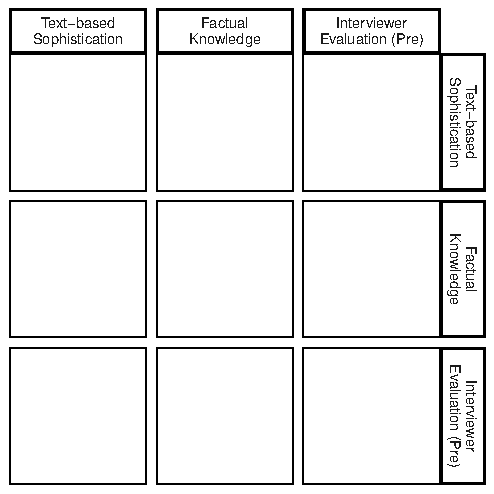
\includegraphics{../fig/corplot_empty.pdf}
  \end{figure}
\end{frame}
\begin{frame} %[allowframebreaks]
\frametitle{Comparison with conventional measures (ANES 2012)}
  \begin{figure}
  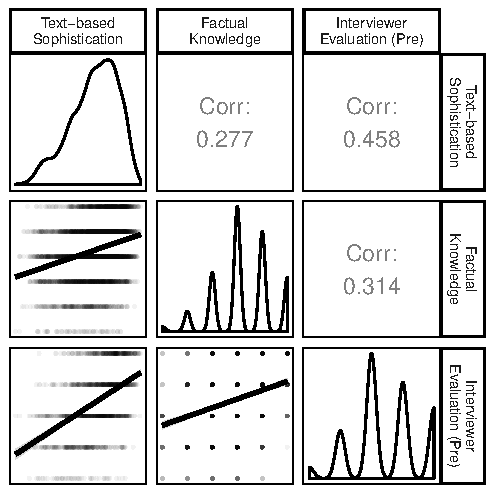
\includegraphics{../fig/corplot_pres.pdf}
  \end{figure}
\end{frame}
% TODO: reduce to text, factual, and interviewer eval (also for the rest...)

\begin{frame} %[allowframebreaks]
\frametitle{Validation: Engagement and participation (ANES 2012)}
  \begin{figure}
  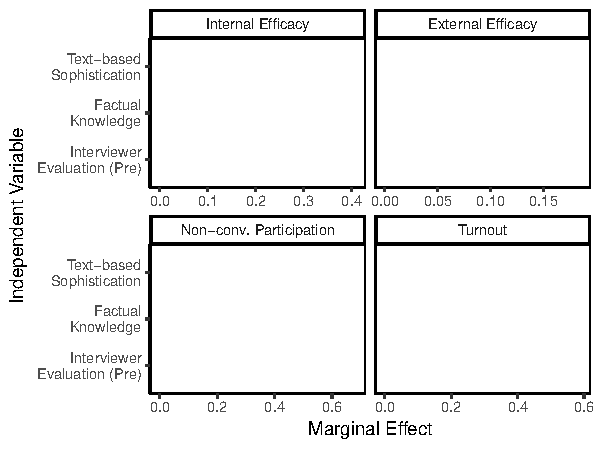
\includegraphics{../fig/knoweff_empty.pdf}
  \end{figure}
\end{frame}
\begin{frame} %[allowframebreaks]
\frametitle{Validation: Engagement and participation (ANES 2012)}
  \begin{figure}
  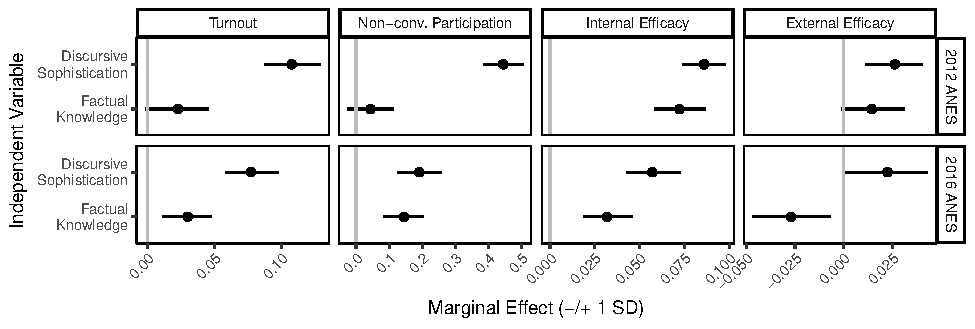
\includegraphics{../fig/knoweff_pres.pdf}
  \end{figure}
\end{frame}

\begin{frame} %[allowframebreaks]
\frametitle{Other validation results}
\begin{itemize}
\item \emph{Text-based sophistication} is associated with \emph{\textbf{...}}
  \begin{enumerate}[\textbf{...}]
  \item<2-> more precise candidate and party \emph{placements} on multiple \emph{policy} issues.
  \item<3-> higher likelihood that citizens \emph{voted} according to their \emph{initial intention} at the time of the \emph{pre-election} interview.
  \item<4-> more accurate \emph{information retrieval} from news articles.
  \item<5-> manual coding of individual \emph{levels of justification} \citep{colombo2016justifications}.
  \end{enumerate}
  \item<6> \emph{But:} conventional measures of \emph{factual knowledge} are, too...
\end{itemize}
\end{frame}

\section{Assessing the gender gap}
% This application challenges a common finding in political science and public opinion research, namely that women know significantly less about politics than men. Some studies attribute this difference to a relative lack in resources like education, or a more general disdain for politics among women. However, others argued that the gender gap might be an artifact due to differential propensities to guess or the fact that knowledge questions do not address gender relevant knowledge. I examine the gender gap by proposing a new measure of political sophistication that focuses on how individuals describe their political attitudes and beliefs in their own words.
% Example for gender gap: Verba, Burns, Schlozman (1997), Mondak


\begin{frame} %[allowframebreaks]
\frametitle{Application: Assessing the gender gap I}
  \begin{figure}
  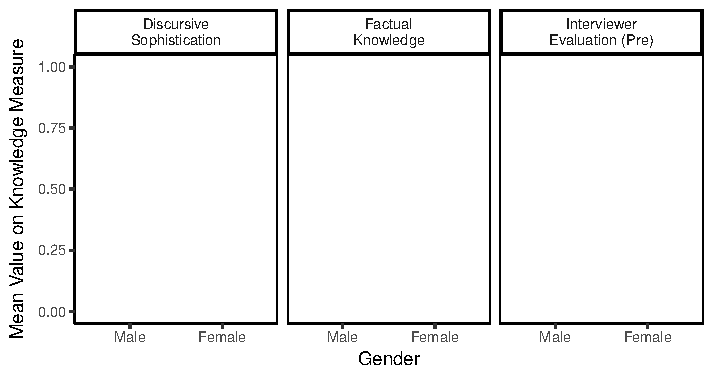
\includegraphics{../fig/meandiff_empty.pdf}
  \end{figure}
\end{frame}
\begin{frame} %[allowframebreaks]
\frametitle{Application: Assessing the gender gap I}
  \begin{figure}
  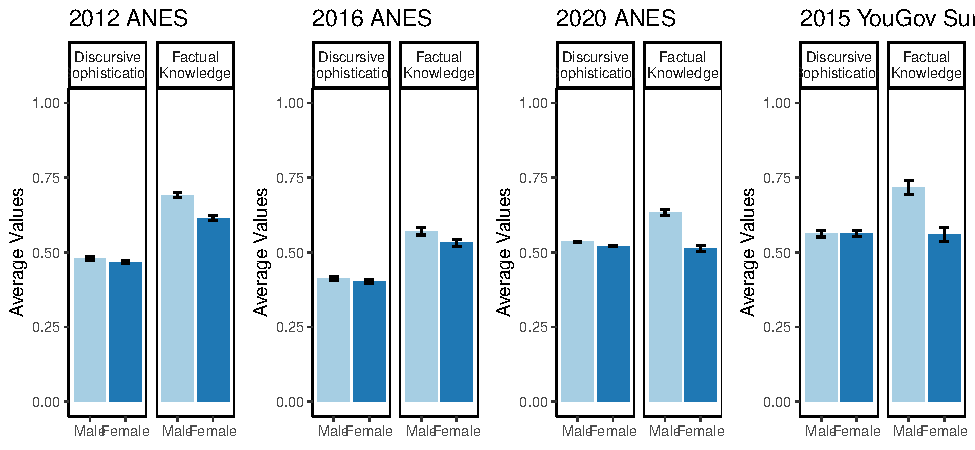
\includegraphics{../fig/meandiff_pres.pdf}
  \end{figure}
\end{frame}

\begin{frame} %[allowframebreaks]
\frametitle{Application: Assessing the gender gap II}
  \begin{figure}
  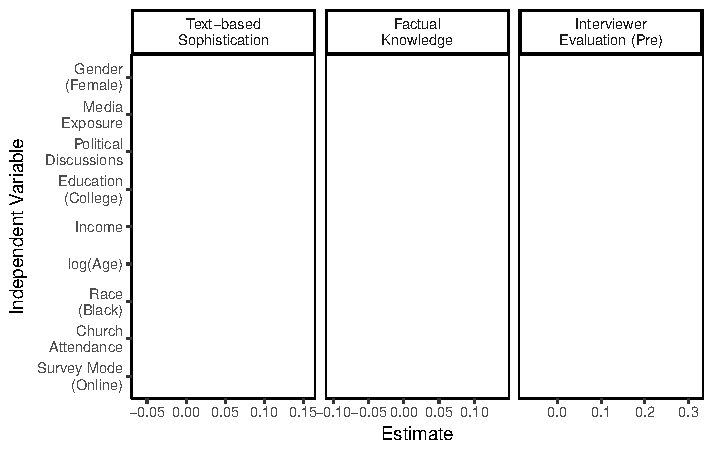
\includegraphics{../fig/determinants_empty.pdf}
  \end{figure}
\end{frame}
\begin{frame} %[allowframebreaks]
\frametitle{Application: Assessing the gender gap II}
  \begin{figure}
  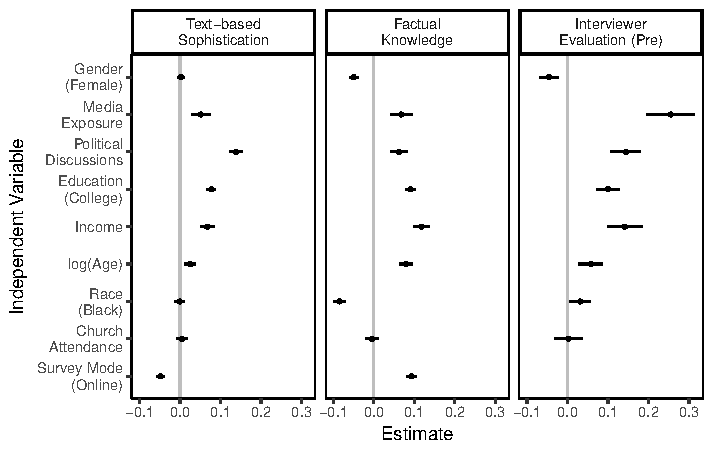
\includegraphics{../fig/determinants_pres.pdf}
  \end{figure}
\end{frame}

%\begin{frame} %[allowframebreaks]
%\frametitle{Closing the Gender Gap}
%  \begin{figure}
%  
\includegraphics[width = \textwidth]{../fig/closing_empty.pdf}
%  \end{figure}
%\end{frame}
%\begin{frame} %[allowframebreaks]
%\frametitle{Closing the Gender Gap}
%  \begin{figure}
%  
\includegraphics[width = \textwidth]{../fig/closing.pdf}
%  \end{figure}
%\end{frame}

% TODO: add the yougov study as a replication

\section{Conclusion}
\subsection{}
\begin{frame}%[allowframebreaks]
  \frametitle{Conclusion}
  \begin{itemize}
\item We observe \emph{theoretically meaningful} variation in the \emph{complexity} of verbatim open-ended responses.
%\item Text-based sophistication and conventional knowledge measures \emph{share a substantial amount of variance}, but they are far from identical.
\item<2->  By directly examining how individuals \emph{justify their attitudes}, we can measure sophistication related to \emph{specific political tasks}.
\item<3-> Text-based sophistication is conceptually closer to the \emph{structure of belief systems} than conventional measures \citep[e.g.,][]{tetlock1983cognitive,luskin1987measuring}.

\hspace{1em}
\item<4-> Women might score lower than men on \emph{factual knowledge} about political institutions, but there are no differences in the \emph{sophistication} of expressed political attitudes.
\end{itemize}
\begin{center}
\visible<5>{\emph{\texttt{\#WomenAlsoKnowStuff}}}
\end{center}
\end{frame}
%Information vs. competence argument by Lupia!!

\begin{frame}%[allowframebreaks]
\frametitle{Who scores higher on political knowledge?}
\begin{table}[ht]\footnotesize\centering
\begin{tabular}{l|p{4.5cm}|p{4.5cm}}
   \toprule
%  & Low Sophistication Response & High Sophistication Response \\ 
    & \textbf{Respondent A} & \textbf{Respondent B} \\ 
    \midrule
  Obama (+) & I think he is honest, has good intentions. & He's got a hot wife. Sound mind. Bill Clinton, the best president we ever had, is voting for him. He's not in any type of scandal and is the perfect president for us now. \\ \hdashline
  Obama (-) & I don't feel he is up for the job, he doesn't really know how to get things accomplished from idea to actual reality. &  \\ \hdashline
  Romney (+) & He comes across as an honest person and I feel that financially he would be better for the country. &  \\ \hdashline
  Romney (-) & I am a moderate conservative and there are some things about anti-gay rights that I don't support. & Everything. \\
    \bottomrule
 \end{tabular}
\end{table}
\end{frame}

% One was a woman, one was a man
% question is: what is more important for competence, factual info about institutions, or the ability to express informed opinions about political actors?

\subsection{}
\begin{frame}%[allowframebreaks]
  \begin{center}
  \large{Thank you very much for your attention!}\\ \vspace{2em}
  Manuscript and code available at:\\
  \emph{\texttt{https://github.com/pwkraft/knowledge}}\\ \vspace{2em}
  Comments, questions?\\
  \emph{\texttt{patrick.kraft@stonybrook.edu}}
  \end{center}
\end{frame}

\subsection{}
\begin{frame}
  \frametitle{References}
  \def\newblock{\hskip .11em plus .33em minus .07em}
  %\nocite{*}
  \begin{scriptsize}
    \bibliographystyle{/data/Dropbox/Uni/Lit/apsr2006}
    \bibliography{/data/Dropbox/Uni/Lit/Literature}
  \end{scriptsize}
\end{frame}

\end{document}